% Five-minute talk: five timed slides (title, question, result, validation, lessons)
% followed by a closing slide and five backup slides (appendix), not timed. Build: ./build.sh
% Every number on the slides is copied from manuscript/numbers.tex,
% short-summary/comparison-numbers.tex or prompts/uso-de-tiempo-y-tokens.md;
% the two derived ones (+31%, 2.3x) are asserted in make_figures.py.
% The ten-minute version is kept in v10min/.
\documentclass[aspectratio=169,11pt]{beamer}
\usetheme[progressbar=frametitle,numbering=fraction]{metropolis}
\usepackage{appendixnumberbeamer}
\usepackage[T1]{fontenc}
\usepackage[utf8]{inputenc}
\usepackage{lmodern}
\usepackage{amsmath}
\usepackage{graphicx}
\usepackage{tikz}
\usetikzlibrary{positioning,arrows.meta}
\graphicspath{{figures/}}

\definecolor{ink}{HTML}{1F2937}
\definecolor{accent}{HTML}{1F5FA8}
\definecolor{warm}{HTML}{D9622B}
\definecolor{muted}{HTML}{6B7280}
\definecolor{paper}{HTML}{FFFFFF}
\setbeamercolor{normal text}{fg=ink,bg=paper}
\setbeamercolor{frametitle}{fg=white,bg=accent}
\setbeamercolor{progress bar}{fg=warm,bg=accent!30}
\setbeamercolor{alerted text}{fg=warm}
\setbeamerfont{frametitle}{size=\large}
\setbeamercolor{block body}{bg=accent!7}

\newcommand{\ext}{\mathsf{ext}}
\newcommand{\GB}{\mathsf{GB}}
\newcommand{\stat}[2]{{\large\bfseries\color{accent}#1\par}\vspace{1pt}{\scriptsize\color{muted}#2\par}}
\newcommand{\src}[1]{{\scriptsize\color{muted}#1}}
\newcommand{\hd}[1]{{\small\bfseries\color{accent}#1}}
\newcommand{\eqbox}[1]{%
  \begin{beamercolorbox}[wd=\linewidth,sep=4pt,center]{block body}#1\end{beamercolorbox}}

\title{Extremality shift of rotating black holes\\at finite Gauss--Bonnet coupling}
\subtitle{A research project carried out with AI agents}

\begin{document}

% ---------------------------------------------------------------- 1  title
\begin{frame}[plain]
\vspace*{0.4cm}
{\LARGE\bfseries\color{accent}Extremality shift of rotating black holes\\[2pt]
at finite Gauss--Bonnet coupling\par}
\vspace{0.25cm}
{\large A research project carried out with AI agents\par}
\vspace{0.55cm}
{\normalsize Cecilia Bejarano$^{1}$, David Blanco$^{2}$, Andrés Goya$^{1}$, Guillem Pérez-Nadal$^{2}$\par}
\vspace{0.12cm}
{\scriptsize\color{muted}$^1$Instituto de Astronomía y Física del Espacio (IAFE, CONICET--UBA)\quad
$^2$Departamento de Física, FCEN--UBA and IFIBA (CONICET--UBA)\par}
\vspace{0.3cm}
{\small With AI assistance: \textbf{Claude Code} (Anthropic; Claude Opus~5, Sonnet~5)
and \textbf{Codex} (OpenAI; GPT-5)\par}
\vfill
{\footnotesize\color{muted}
\emph{Gravitational Waves and AI-Assisted Research} --- M.~Zaldarriaga \& N.~Mirón-Granese\\
Departamento de Física, FCEN, Universidad de Buenos Aires \quad·\quad 2 October 2026
\quad·\quad \texttt{github.com/ddblanco/BHs}\par}
\end{frame}

% ---------------------------------------------------------------- 2  problem
\begin{frame}{The question: how far does Gauss--Bonnet move the spin bound?}
\begin{columns}[T,onlytextwidth]
\column{.33\textwidth}\centering
\vspace{10pt}
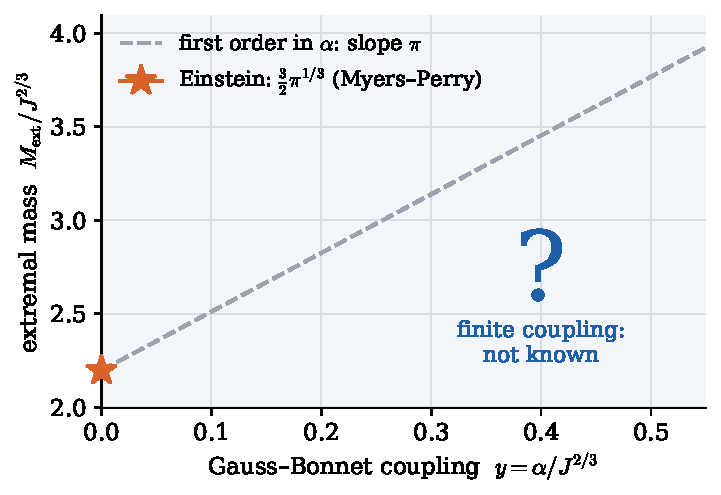
\includegraphics[width=\linewidth]{fig-question.pdf}
\column{.64\textwidth}\small
\setlength{\abovedisplayskip}{3pt}\setlength{\belowdisplayskip}{5pt}
\hd{General Relativity} \src{(in 5D, two equal spins $J_1=J_2=J$)}
\par\smallskip
\noindent\hspace*{.6em}\mbox{Kerr (4D): \ $M^2\ge|J|$ \quad Myers--Perry (5D): \ $M\ge\tfrac32\,\pi^{1/3}J^{2/3}$}\par\smallskip
\hspace*{.6em}\alert{extremal case:} bound saturates $\rightarrow$ \ $T=0$\par
\medskip
\hd{Add Gauss--Bonnet term}, coupling $\alpha$:
\[I=\tfrac1{16\pi G}\!\int\!\sqrt{-g}\,\bigl(R+\alpha\,\mathcal L_{\GB}\bigr)\]
\hd{Known} to first order in $\alpha$ \src{(arXiv:2009.00015)}:
\[M_\ext=\tfrac32\pi^{1/3}J^{2/3}+\pi\,\alpha+\mathcal O(\alpha^2)\]
\hd{Asked:} \ $\partial M_\ext/\partial\alpha|_J$ at \alert{finite} $\alpha$?
\end{columns}
\end{frame}

% ---------------------------------------------------------------- 3  result
\begin{frame}{Main result: the bound tightens, but not linearly}
\vspace{-4pt}
\begin{center}
\begin{tabular}{@{}c@{\hspace{2.2em}}c@{\hspace{2.2em}}c@{}}
{\scriptsize\color{muted}extended first law} &
{\scriptsize\color{muted}at $T=0$, fixed $J$} &
{\scriptsize\color{muted}slope of the extremal mass}\\[2pt]
$\displaystyle dM=T\,dS+2\,\Omega_H\,dJ+\alert{\Psi}\,d\alpha$ &
$\displaystyle\Longrightarrow$ &
$\displaystyle\frac{\partial M_\ext}{\partial\alpha}\bigg|_J=\alert{\Psi_\ext}$
\end{tabular}
\end{center}
\vspace{-2pt}
\begin{columns}[T,onlytextwidth]
\column{.47\textwidth}\centering\vspace{0pt}
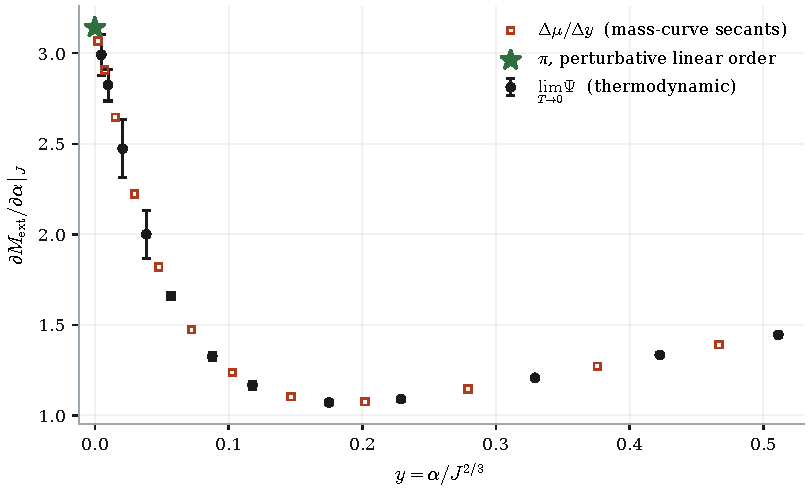
\includegraphics[width=.94\linewidth]{fig-shift.pdf}\\[-2pt]
\scriptsize slope $\partial M_\ext/\partial\alpha|_J$ \ (\alert{result})
\column{.30\textwidth}\centering\vspace{0pt}
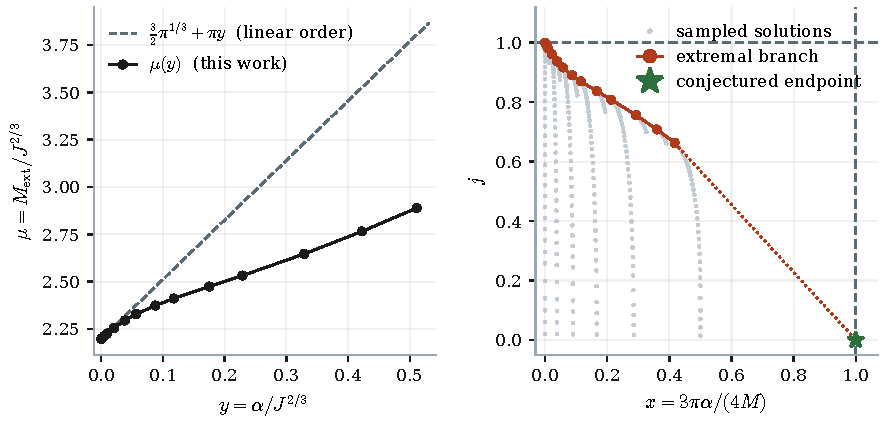
\includegraphics[width=\linewidth,trim=0 0 208.1bp 0,clip]{fig-massext.pdf}\\[-2pt]
\scriptsize extremal mass
\column{.19\textwidth}\raggedright\vspace{8pt}
\stat{$>0$}{bound tightens}\vspace{2pt}
{\normalsize\bfseries\color{accent}$\pi\!\to\!1.07\!\to\!1.44$\par}\vspace{1pt}{\scriptsize\color{muted}not monotonic\par}\vspace{2pt}
\stat{$+31\%$}{growth of $M_\ext$}\vspace{2pt}
\stat{$2.3\times$}{first-order shift vs.\ measured}
\end{columns}
\vfill
\centering\src{356 numerical solutions at 13 couplings; the $T=0$ values are extrapolated from $TJ^{1/3}\approx3\times10^{-6}$.}
\end{frame}

% ---------------------------------------------------------------- 4  validation
\begin{frame}{Validation: how do we know it is right?}
\begin{columns}[T,onlytextwidth]
\column{.57\textwidth}\centering
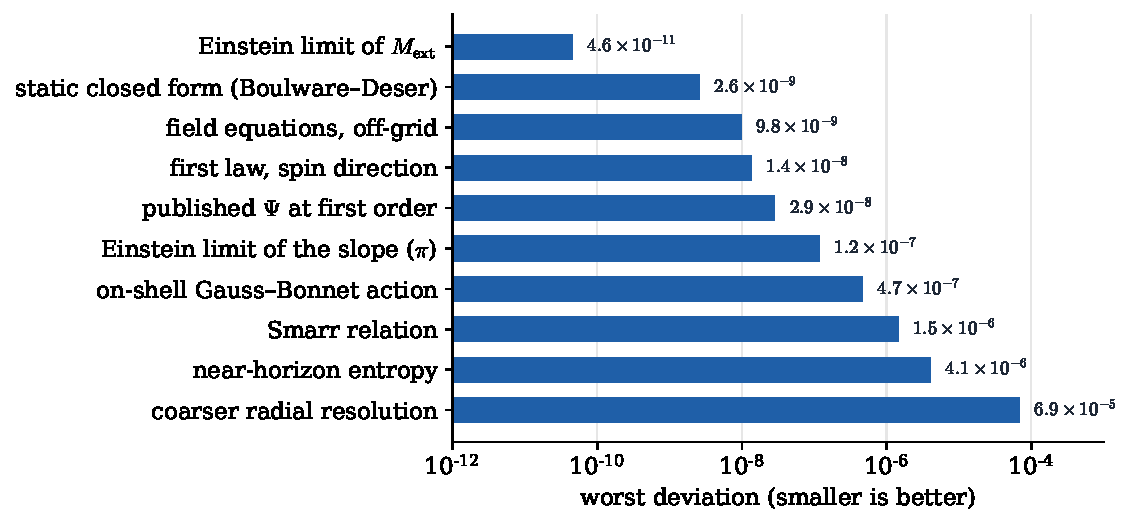
\includegraphics[width=\linewidth]{fig-checks.pdf}\\
\src{worst deviation of each independent check}
\column{.40\textwidth}\footnotesize
\setlength{\abovedisplayskip}{2pt}\setlength{\belowdisplayskip}{2pt}
\hd{1. Known answers first}\\
published family (arXiv:1010.0860) to $2\times10^{-4}$;
static closed form; $\pi$ at $\alpha\to0$

\smallskip
\hd{2. Independent routes to $\Psi$}\\
Smarr, from one solution's charges:
\[\Psi=\frac{2M-3TS-6\Omega_HJ}{2\alpha}\]
on-shell Gauss--Bonnet action:
\[\Psi=-\frac1{16\pi}\int_\Sigma\!\sqrt{-g}\,\mathcal L_{\GB}\]
neither uses our linear solve: agree to $\sim10^{-6}$

\smallskip
\hd{3. Largest uncertainty}\\
$T\to0$ is an extrapolation (the error bars)
\end{columns}
\end{frame}

% ---------------------------------------------------------------- 5  experience
\begin{frame}{What we learned working with agents}
\begin{columns}[T,onlytextwidth]
\column{.46\textwidth}\centering
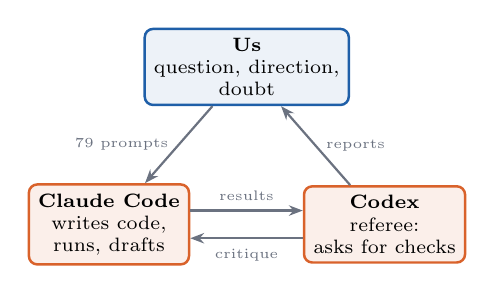
\begin{tikzpicture}[
  every node/.style={font=\scriptsize,align=center,rounded corners=3pt,
                     draw=accent,line width=0.9pt,fill=accent!8,minimum width=1.9cm,minimum height=0.9cm},
  hot/.style={draw=warm,fill=warm!10},
  lab/.style={draw=none,fill=none,font=\tiny\color{muted},minimum width=0,minimum height=0},
  >={Stealth[length=5pt]}]
\node (h) {\textbf{Us}\\question, direction,\\doubt};
\node[hot] (c) at (-1.75,-2.0) {\textbf{Claude Code}\\writes code,\\runs, drafts};
\node[hot] (x) at (1.75,-2.0) {\textbf{Codex}\\referee:\\asks for checks};
\draw[->,thick,muted] (h) -- node[lab,left]{79 prompts} (c);
\draw[->,thick,muted] ([yshift=5pt]c.east) -- node[lab,above]{results} ([yshift=5pt]x.west);
\draw[->,thick,muted] ([yshift=-5pt]x.west) -- node[lab,below]{critique} ([yshift=-5pt]c.east);
\draw[->,thick,muted] (x) -- node[lab,right]{reports} (h);
\end{tikzpicture}

\vspace{6pt}
\raggedright\scriptsize
A check the referee asked for \alert{failed}; an exact bound caught a real mass error.
\column{.52\textwidth}\centering
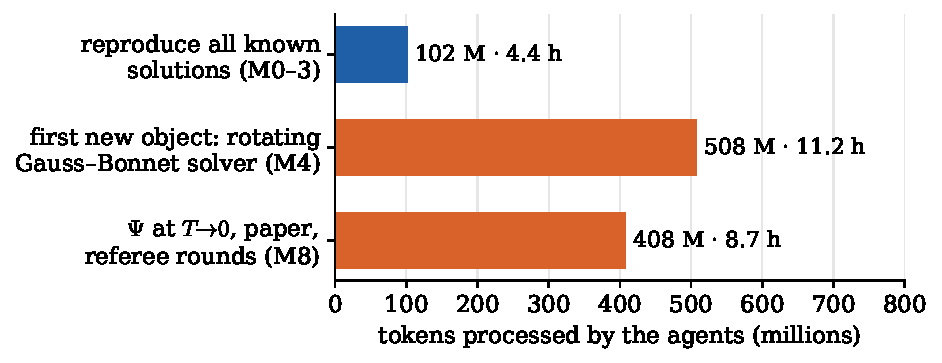
\includegraphics[width=\linewidth]{fig-effort.pdf}

\vspace{4pt}
\begin{columns}[T,onlytextwidth]
\column{.5\linewidth}\centering\stat{36.8 h}{agent time over 13 days}
\column{.5\linewidth}\centering\stat{1.42 billion}{tokens processed}
\end{columns}
\end{columns}
\vfill
\centering\small
\textbf{Lesson:} the cost is not writing code, it is verifying it.\\
Ask for checks that \alert{can fail}, and let one agent referee the other.
\end{frame}

% ---------------------------------------------------------------- 6  thanks
\begin{frame}[standout]
Thank you for your attention\\[14pt]
{\normalsize\mdseries Thanks Matías and Nahuel for the AI course}
\end{frame}

% ================================================================ backup
\appendix

% ---------------------------------------------------------------- A1
\begin{frame}{A1 · Numerical method: solving the field equations}
\vspace{-6pt}
\begin{columns}[T,onlytextwidth]
\column{.53\textwidth}\scriptsize
\setlength{\abovedisplayskip}{1pt}\setlength{\belowdisplayskip}{1pt}
{\bfseries\color{accent}Equal-spin ansatz} $\Rightarrow$ ODEs in $r$ for $b,f,h,w$:
\[\begin{aligned}ds^2={}&-b\,dt^2+\frac{dr^2}{f}+r^2\bigl[d\theta^2+\sin^2\!\theta\cos^2\!\theta\,(d\varphi_1-d\varphi_2)^2\bigr]\\
&+h\,\bigl[\sin^2\!\theta\,d\varphi_1+\cos^2\!\theta\,d\varphi_2-w\,dt\bigr]^2\end{aligned}\]
horizon: $b=f=0$, $w=\Omega_H$;\ \ infinity: $b,f,h/r^2\to1$, $w\to0$\par
\column{.45\textwidth}\scriptsize
{\bfseries\color{accent}Discretise:} $\chi=1-r_H/r$, Chebyshev--Lobatto, $N=64$:
$R_N(u;\alpha,r_H,\Omega_H)=0$ \ ($4N$ eqs.)\\[2pt]
{\bfseries\color{accent}Solve:} damped Newton; continuation from Myers--Perry\\[2pt]
{\bfseries\color{accent}Accept:} $G_{\mu\nu}+\alpha H_{\mu\nu}<10^{-8}$ at 51 off-grid points\\[2pt]
{\bfseries\color{accent}Read off:} $b\simeq1+U/r^2$, $w\simeq W/r^4$ $\Rightarrow$ $M=-\tfrac{3\pi}8U$, $J=\tfrac\pi4W$
\end{columns}
\vspace{4pt}
\begin{columns}[T,onlytextwidth]
\column{.43\textwidth}\centering
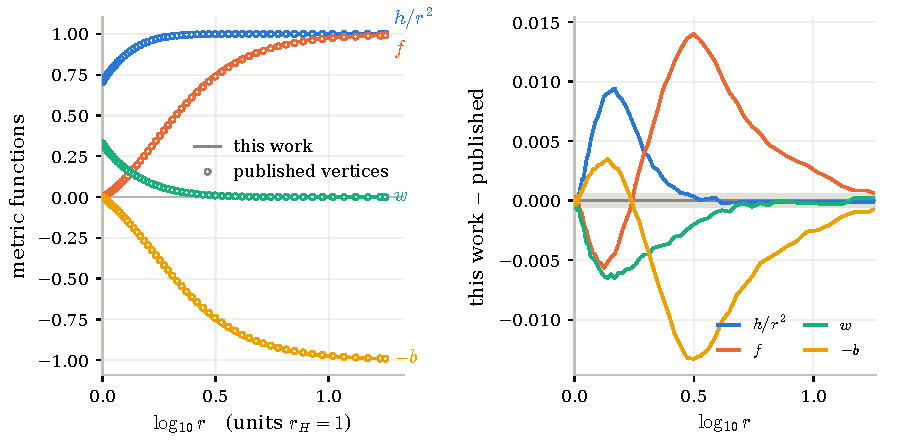
\includegraphics[height=3.6cm,trim=0 0 217bp 0,clip]{fig-paper-comparison.pdf}
\column{.55\textwidth}\centering
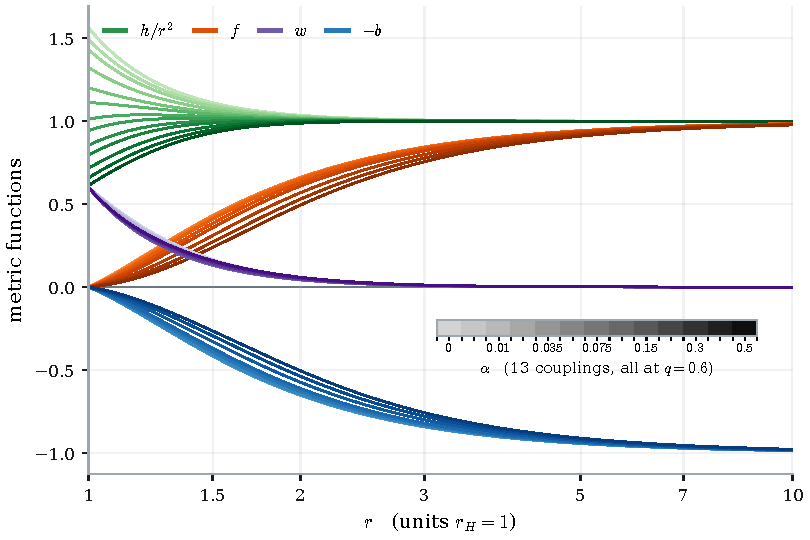
\includegraphics[height=3.6cm]{fig-profiles.pdf}
\end{columns}
\end{frame}

% ---------------------------------------------------------------- A2
\begin{frame}{A2 · Numerical method: measuring $\Psi$ and reaching $T=0$}
\begin{columns}[T,onlytextwidth]
\column{.47\textwidth}\small
\hd{$\Psi$ from derivatives at fixed $(r_H,\Omega_H)$}
\[\Psi=\left.\frac{\partial M}{\partial\alpha}\right|_{S,J}=M_\alpha-T\,S_\alpha-2\Omega_H\,J_\alpha\]

\hd{Derivatives without finite differences}
\[\underbrace{\frac{\partial R_N}{\partial u}}_{\text{Newton Jacobian}}\frac{du}{d\alpha}=-\frac{\partial R_N}{\partial\alpha}\]
\scriptsize one linear solve, no step size (implicit function theorem)

\medskip\small
\hd{Get cold, then extrapolate}\\
cubic fit through the 6 coldest states;\\
coldest $TJ^{1/3}\approx3\times10^{-6}$
\column{.51\textwidth}\centering
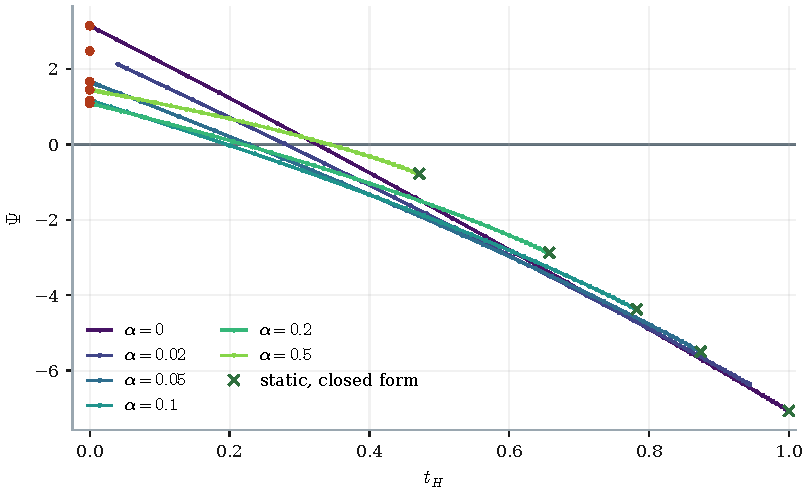
\includegraphics[width=\linewidth]{fig-potential.pdf}\\
\scriptsize $\Psi$ against temperature; red dots: the $T=0$ values (the slope)
\end{columns}
\end{frame}

% ---------------------------------------------------------------- A3
\begin{frame}{A3 · Physical meaning of the result}
\centering
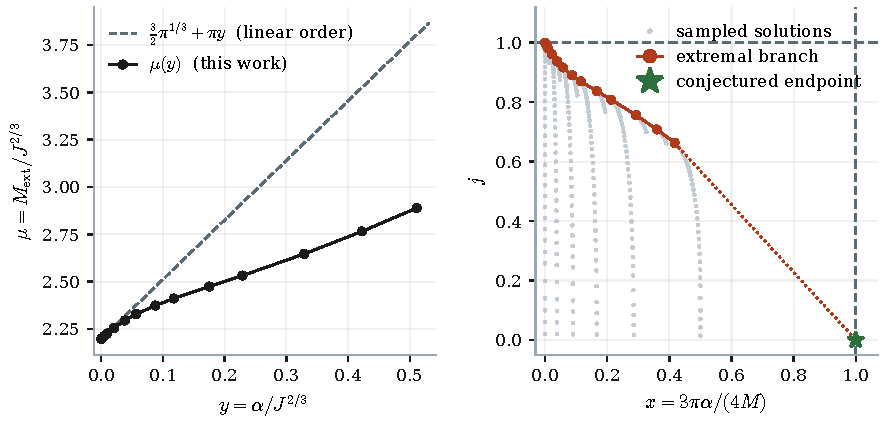
\includegraphics[width=.66\textwidth]{fig-massext.pdf}

\vspace{2pt}
\begin{columns}[T,onlytextwidth]
\column{.34\textwidth}\centering\small
\hd{Spin bound}\\
$\Psi_\ext>0\ \Leftrightarrow\ j_\ext$ falls:\\
less spin per unit mass
\column{.32\textwidth}\centering\small
\hd{Slope minimum}\\
$3\omega=\mu-y\,\mu'$\\
= fastest extremal horizon,\\ $\omega=\Omega_HJ^{1/3}$
\column{.34\textwidth}\centering\small
\hd{Why it rises again}\\
$M>\tfrac{3\pi}4\alpha$ \ forces\\
$\mu'\to\tfrac{3\pi}{4}\approx2.36$
\end{columns}
\end{frame}

% ---------------------------------------------------------------- A4
\begin{frame}[t]{A4 · How it started: the first prompts}
\vspace{-4pt}
\begin{beamercolorbox}[wd=\linewidth,sep=4pt,leftskip=4pt]{block body}
\scriptsize\itshape ``El proyecto consiste en utilizar agentes de IA para implementar códigos
numéricos que permitan obtener soluciones de agujeros negros rotantes en
dimensión D>4 [\ldots] reproducir soluciones numéricas ya encontradas en la
literatura. [\ldots] el paso siguiente sería emprender la búsqueda de nuevas
soluciones.''\par\smallskip\upshape\tiny\color{muted}Prompt 1 --- 4 Sept, 19:16, to Codex
\quad·\quad then ``Fijate que el proyecto realmente siga las indicaciones propuestas por el
docente del curso'' (3), ``ejecutar con subagentes'' (5), ``continuemos con el hito 3'', ``dale, avanzá''
\quad·\quad \textbf{79} human prompts, 4--28 Sept \quad·\quad Claude Code builds $\leftrightarrow$ Codex referees
\end{beamercolorbox}
\par\vspace{-16pt}\noindent
\begin{minipage}[t]{.44\textwidth}\vspace{0pt}\centering
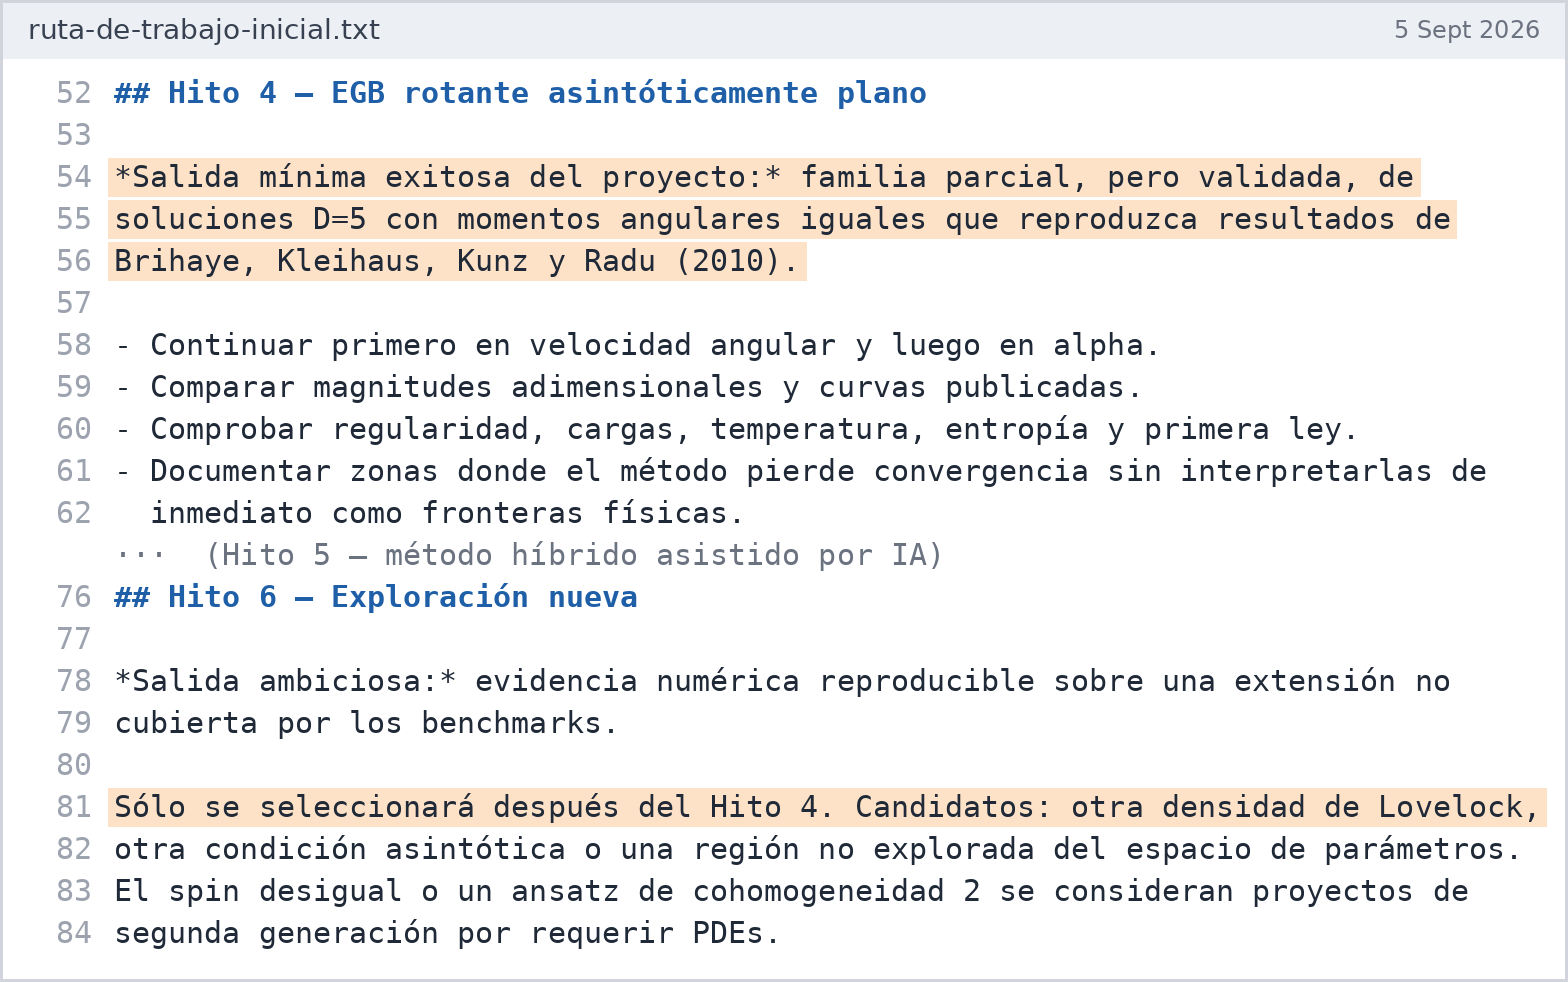
\includegraphics[width=.9\linewidth]{fig-roadmap.png}\par\vspace{2pt}
{\tiny\color{muted}first roadmap, 5 Sept. \textcolor{warm}{Hito 6} became $\Psi$;
Hito 8 ($T\to0$, paper, referees) was not in the plan.\par}
\end{minipage}\hfill
\begin{minipage}[t]{.52\textwidth}\vspace{0pt}\centering
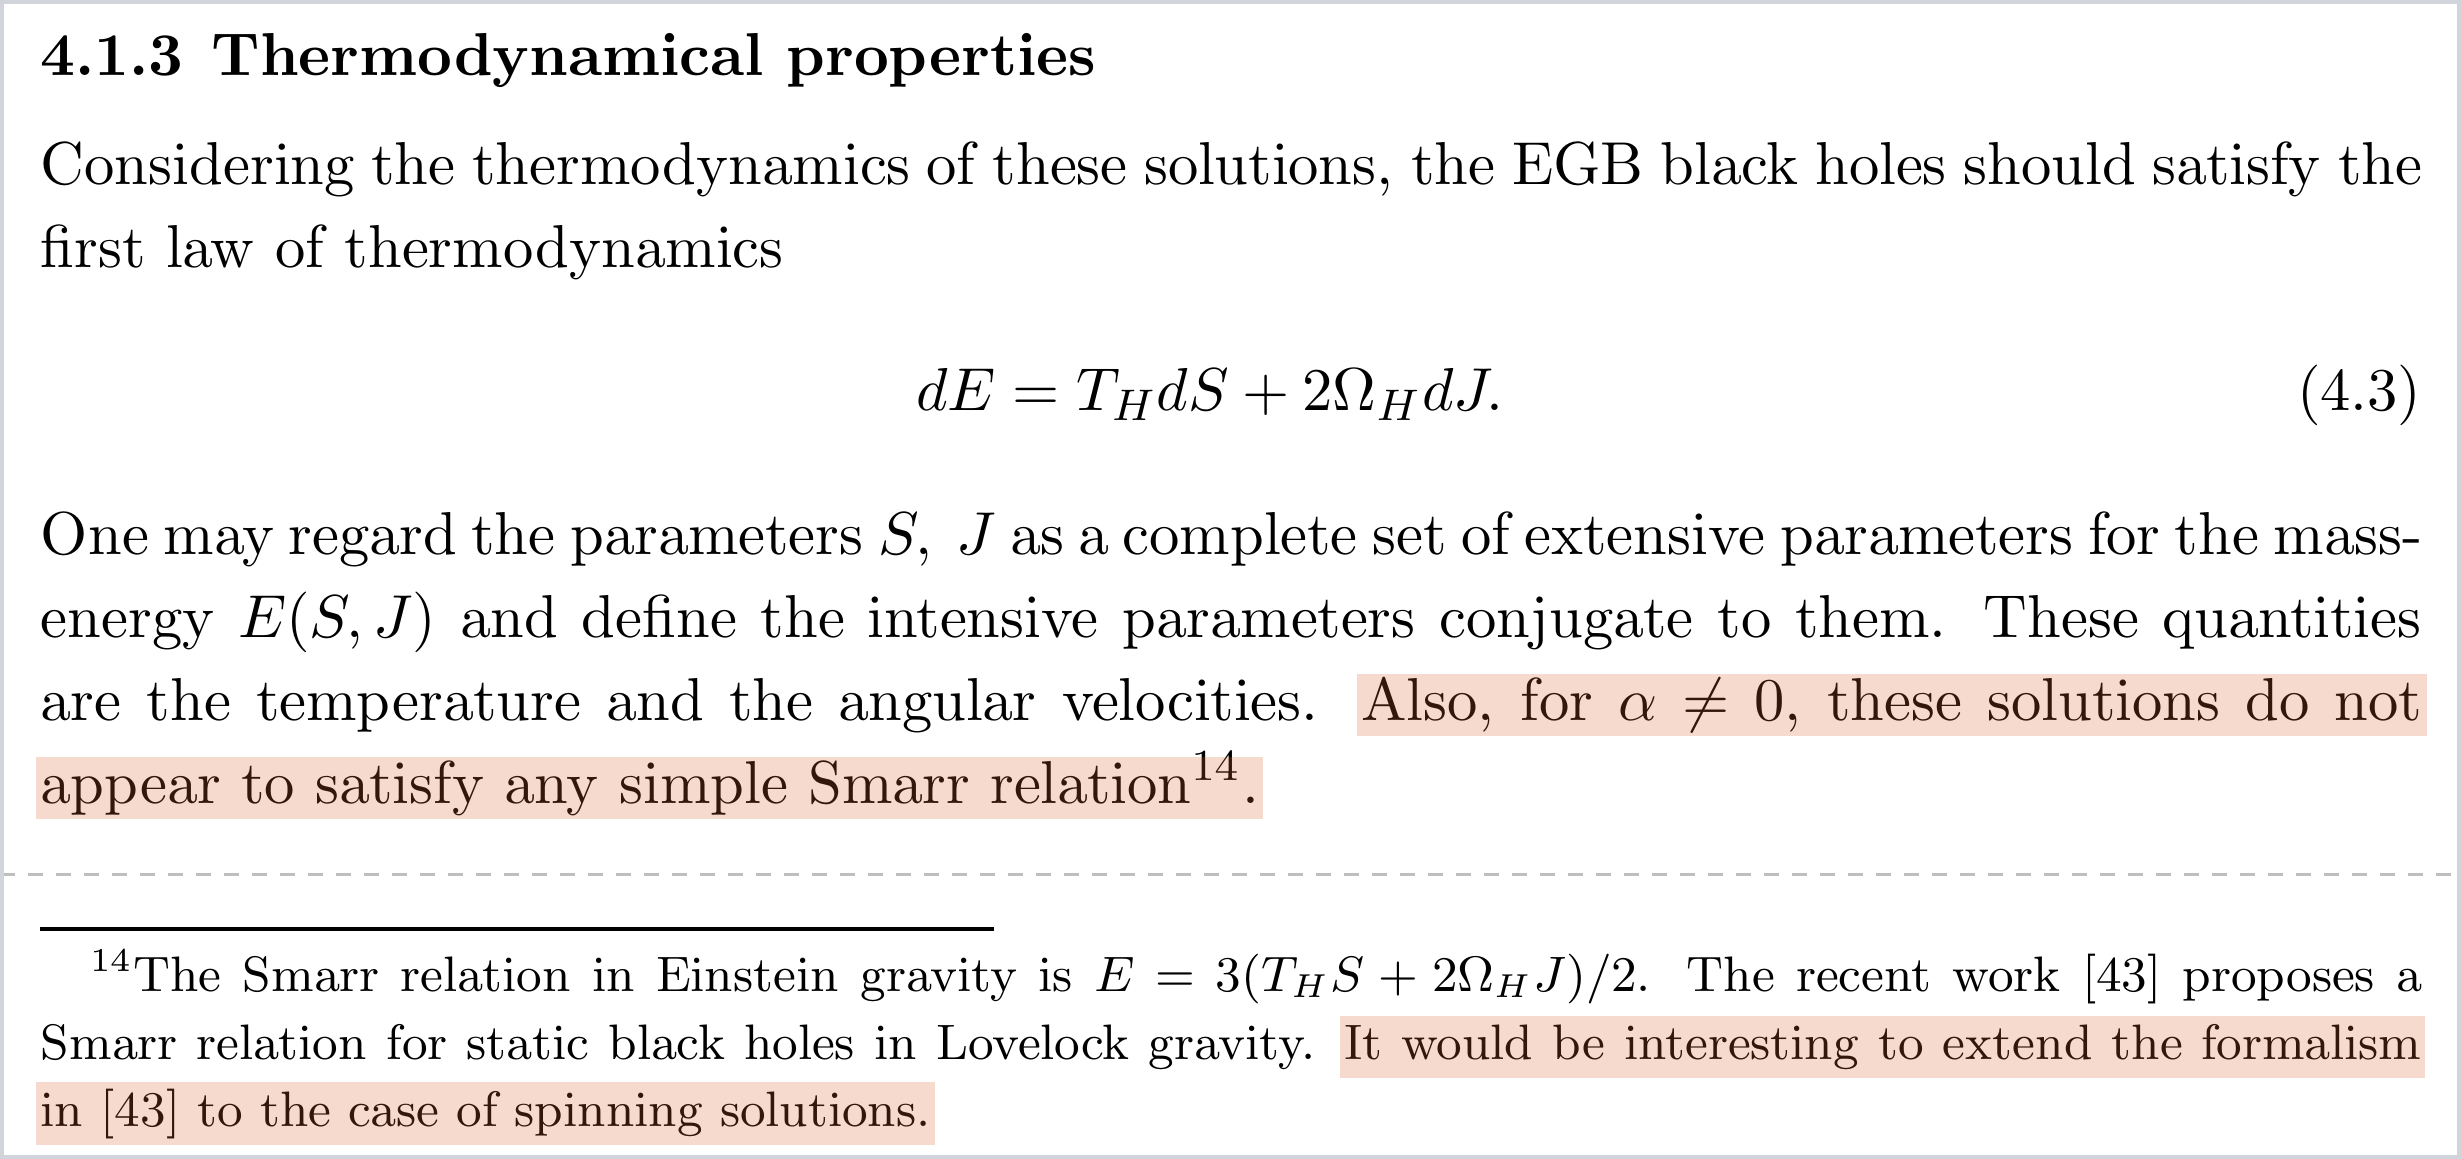
\includegraphics[width=\linewidth]{fig-smarr.png}\par\vspace{2pt}
{\tiny\color{muted}arXiv:1010.0860, \S4.1.3 and footnote 14.\par}
\vspace{4pt}
{\scriptsize Hito 6, $\alpha$ as a thermodynamic variable:\
$2M=3TS+6\Omega_HJ+2\alpha\Psi$\par}
\end{minipage}
\end{frame}

% ---------------------------------------------------------------- A5
\begin{frame}{A5 · What it cost}
\centering
\begin{columns}[T,onlytextwidth]
\column{.25\textwidth}\centering\stat{36.8 h}{active agent time, 13 days}
\column{.25\textwidth}\centering\stat{1.42 billion}{tokens processed\\(99\% re-read context)}
\column{.25\textwidth}\centering\stat{5.9 million}{tokens written ($\approx$24 MB)}
\column{.25\textwidth}\centering\stat{79}{human prompts}
\end{columns}
\vspace{4pt}
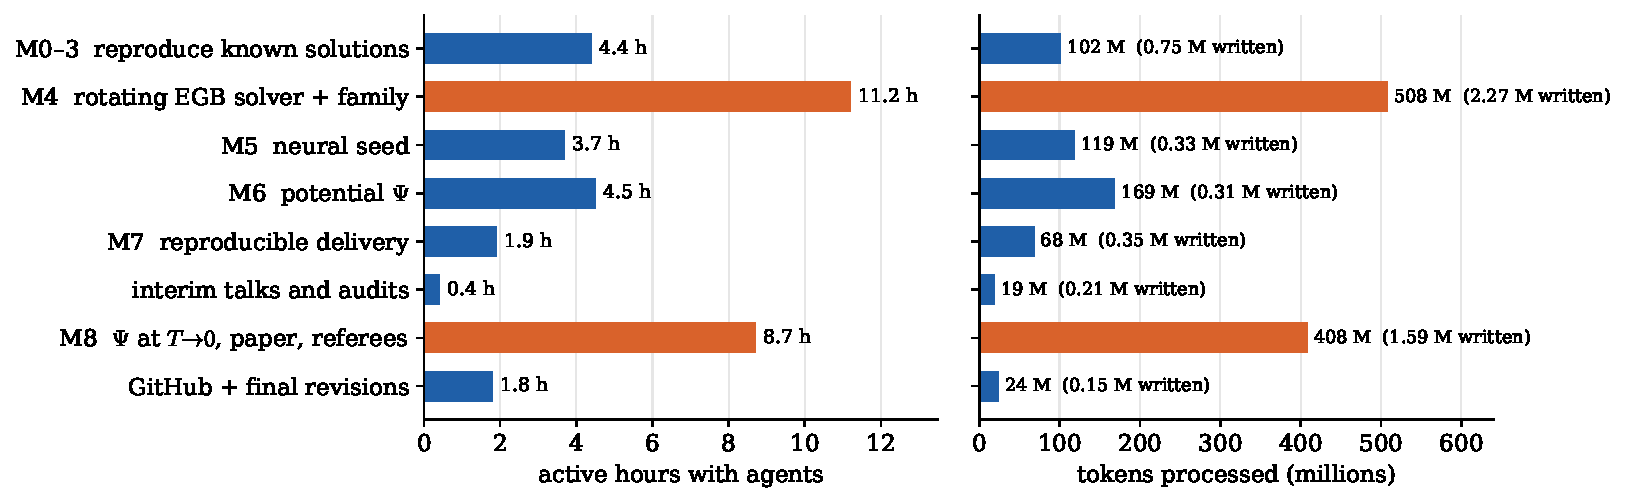
\includegraphics[width=.8\textwidth]{fig-cost.pdf}\\
\small The first \alert{new} object cost $5\times$ the tokens of reproducing everything known.\\[2pt]
\src{Not counted: human time, background numerical runs.}
\end{frame}

\end{document}
